% Generated by book/tools/notebook_to_tex.py. Do not edit by hand.

\chapter[BERT 다중 클래스 분류 (Multi-class \& CE)]{BERT 다중 클래스 분류 (Multi-class \& CE)}

\label{ch:12}

\markboth{BERT 다중 클래스 분류 (Multi-class \& CE)}{BERT 다중 클래스 분류 (Multi-class \& CE)}

\chaptermeta{12_bert_multiclass/12_bert_multiclass.ipynb}{https://colab.research.google.com/github/yoon-gu/neuqes-101/blob/master/12_bert_multiclass/12_bert_multiclass.ipynb}{Yelp 5클래스 분류로 확장한 DistilBERT softmax 분류}



\index{1BERT multi class classification@BERT multi-class classification}

\index{1multi class classification@multi-class classification}

\index{1CrossEntropyLoss@CrossEntropyLoss}

\index{1num labels 5@num\_labels=5}

\index{1confusion matrix@confusion\_matrix}

\index{1classification report@classification\_report}

\index{1roc auc score@roc\_auc\_score}

\index{1macro F1@macro F1}

\index{1calibration@calibration}

\index{1random baseline@random baseline}

\index{0다중 클래스 분류@다중 클래스 분류}

\index{0혼동 행렬@혼동 행렬}

\index{0분류 리포트@분류 리포트}

\index{0매크로 F1@매크로 F1}

\index{0캘리브레이션@캘리브레이션}

\index{0랜덤 기준선@랜덤 기준선}

\index{1seaborn heatmap@seaborn.heatmap}

\index{1row normalized confusion matrix@row-normalized confusion matrix}

\index{1multi class AUC@multi-class AUC}

\index{1top 1 probability@top-1 probability}

\index{1log K baseline@log K baseline}

\index{1ordinal label@ordinal label}

\index{0행 정규화 혼동 행렬@행 정규화 혼동 행렬}

\index{0다중 클래스 AUC@다중 클래스 AUC}

\index{0최상위 확률@최상위 확률}

\index{0순서형 라벨@순서형 라벨}



\section{변화추적표}

\begin{booktable}{12장 변화추적표}{tab:ch12-01}
\begin{adjustbox}{max width=\textwidth}
\begin{tabular}{@{}lllllll@{}}
\toprule
Ch & 모델 & 토크나이저 & 데이터 & Output Head & Activation & Loss \\
\midrule

5 & \inlinecode{LogisticRegression(multinomial)} & \inlinecode{TfidfVectorizer()} & Yelp 5클래스 & (5차원) & softmax & \inlinecode{CrossEntropyLoss} \\
11 & DistilBERT 파인튜닝 & \inlinecode{AutoTokenizer.from\_pretrained(...)} & Yelp 이진화 & \inlinecode{Linear(H,\ 2)} & softmax & \inlinecode{CrossEntropyLoss} \\
\textbf{12 ← 여기} & DistilBERT 파인튜닝 & 같음 & \textbf{Yelp 5클래스} & \textbf{\inlinecode{Linear(H,\ 5)}} & softmax & \inlinecode{CrossEntropyLoss} \\
13 (다음) & DistilBERT 파인튜닝 & 같음 & Yelp + 측면 키워드 (5라벨 multi-label) & \inlinecode{Linear(H,\ 5)} & sigmoid (per-label) & \inlinecode{BCEWithLogitsLoss} (per-label) \\
\bottomrule
\end{tabular}
\end{adjustbox}
\end{booktable}

전체 20장 표는 \href{https://github.com/yoon-gu/neuqes-101\#챕터별-변화추적표}{루트 README.md}를 참고하세요.



\section{변경점: \ref{ch:11}장 대비}

\begin{booktable}{12장 변경점 요약}{tab:ch12-02}
\begin{adjustbox}{max width=\textwidth}
\begin{tabular}{@{}lll@{}}
\toprule
축 & \ref{ch:11}장 (binary) & \ref{ch:12}장 (multi-class) \\
\midrule

\textbf{Task} & 이진 분류 & \textbf{5-클래스 분류} ← \emph{유일한 변화} \\
\inlinecode{num\_labels} & 2 & \textbf{5} \\
데이터 & Yelp 이진화 (별점 3 제외) & \textbf{Yelp 별점 1-5 그대로} (제외 없음) \\
라벨 형식 & int \inlinecode{0} / \inlinecode{1} & \textbf{int \inlinecode{0}-\inlinecode{4}} (별점-1) \\
\inlinecode{problem\_type} & \inlinecode{single\_label\_classification} & (그대로) \\
Activation / Loss & softmax / CE & (그대로) \\
평가 metric & binary precision/recall/F1 + AUC & \textbf{accuracy + macro precision/recall/F1 + multi-class AUC (OvR)} \\
학습 hyperparams (lr, batch, epoch, seed) & 동일 & 동일 \\
\bottomrule
\end{tabular}
\end{adjustbox}
\end{booktable}

\begin{quote}
\textbf{변경점 한 가지 원칙}: Loss·activation·문제 셋업이 그대로 유지되고 \emph{task 차원만 K=2 → K=5} 로 일반화됩니다. \ref{ch:05}장의 sklearn 장에서 본 K=5 셋업이 BERT에 그대로 옮겨오는 모습을 확인하는 것이 핵심.
\end{quote}



\section{\texorpdfstring{손실 노트}{손실 노트}}

수식은 \ref{ch:04}--\ref{ch:05}장·11과 동일:

\begin{equation}
\label{eq:ch12-01}
L = -\frac{1}{N}\sum_{i=1}^{N}\log \hat p_{i, y_i} \quad\text{where}\quad \hat p_{i,k} = \dfrac{e^{z_{i,k}}}{\sum_{j=1}^{K} e^{z_{i,j}}}
\end{equation}

식~\eqref{eq:ch12-01}은 이 절에서 사용하는 핵심 관계를 정리한 것입니다.

K가 늘어나면 \emph{random baseline 손실} 도 같이 커집니다 --- 학습 초반 모델이 logit을 거의 0으로 출력하면 softmax는 균등 \((1/K, \ldots, 1/K)\) 가 되고 정답 클래스의 손실은 \(-\log(1/K) = \log K\).

\begin{booktable}{12장 손실 노트 표}{tab:ch12-03}
\begin{adjustbox}{max width=\textwidth}
\begin{tabular}{@{}lll@{}}
\toprule
K & random baseline loss \(-\log(1/K)\) & 의미 \\
\midrule

2 & \(\log 2 = 0.693\) & \ref{ch:11}장 학습 첫 step에서 흔히 보이는 값 \\
5 & \(\log 5 = 1.609\) & \textbf{이 장 학습 첫 step의 baseline} \\
10 & \(\log 10 = 2.303\) & 일반적인 ImageNet 1000클래스 학습 비교 \\
1000 & \(\log 1000 = 6.908\) & 학습 시작 직후 손실이 \textasciitilde7이면 정상 \\
\bottomrule
\end{tabular}
\end{adjustbox}
\end{booktable}

\textbf{숫자로 감 잡기 (K=5, 정답=클래스 4)} --- logits에서 정답 클래스가 얼마나 커야 손실이 얼마인지:

\begin{booktable}{12장 손실 노트 표}{tab:ch12-04}
\begin{adjustbox}{max width=\textwidth}
\begin{tabular}{@{}lll@{}}
\toprule
logits \((z_0, z_1, z_2, z_3, z_4)\) & softmax → \(\hat p_4\) & 손실 \(-\log \hat p_4\) \\
\midrule

\((0, 0, 0, 0, 0)\) & \(0.200\) & \textbf{1.609} ← random \\
\((0, 0, 0, 0, 2)\) & \(0.541\) & 0.615 \\
\((0, 0, 0, 0, 5)\) & \(0.985\) & 0.015 \\
\((5, 0, 0, 0, 0)\) & \(0.005\) & \textbf{5.310} ← 자신 있게 틀린 케이스 \\
\bottomrule
\end{tabular}
\end{adjustbox}
\end{booktable}

\textbf{핵심 직감 --- softmax는 \emph{상대 logit} 만 본다}: 모든 logit에 같은 상수를 더해도 softmax는 변하지 않음 (\(e^{z_k+c} / \sum e^{z_j+c} = e^{z_k}/\sum e^{z_j}\)). 즉 K=5 모델이 학습할 때 의미 있는 신호는 \emph{클래스 간 logit 차이} 뿐. \emph{softmax의 4가지 자유도} (K=5에서 K-1=4)만 학습됨.



\section{토크나이저 노트}

\ref{ch:11}장과 완전히 동일 --- \inlinecode{distilbert-base-uncased} WordPiece, \inlinecode{max\_length=128}. 토크나이저는 라벨 개수에 상관없이 \emph{문장} 만 처리하므로 K가 2든 5든 변화 없습니다. 라벨 개수는 모델의 \emph{분류 헤드} 와 \emph{데이터 라벨 형식} 에서만 다릅니다.

\begin{previewBox}{미리보기}
\textbf{다음 장(\ref{ch:13}장)}: 토크나이저 동일. 변하는 건 \emph{라벨 형식} (int 인덱스 → multi-hot 벡터)과 그에 따른 활성화·loss(softmax/CE → sigmoid/BCE per-label).
\end{previewBox}



\Needspace{8\baselineskip}
\begin{lstlisting}
!pip install -q transformers datasets
\end{lstlisting}

\begin{codeRead}
\textbf{1행}의 \inlinecode{!pip install -q transform...}에서는 Colab 실행에 필요한 패키지를 설치합니다.
\end{codeRead}



\Needspace{26\baselineskip}
\begin{lstlisting}
import warnings
warnings.filterwarnings("ignore")

import numpy as np
import pandas as pd
import matplotlib.pyplot as plt
import seaborn as sns
import torch
from datasets import load_dataset
from transformers import (
    AutoTokenizer, AutoModelForSequenceClassification,
    Trainer, TrainingArguments,
)
from sklearn.metrics import (
    accuracy_score, precision_recall_fscore_support,
    classification_report, roc_auc_score, confusion_matrix,
)

from sklearn.feature_extraction.text import TfidfVectorizer
from sklearn.linear_model import LogisticRegression

plt.rcParams["axes.unicode_minus"] = False

print(f"PyTorch:        {torch.__version__}")
print(f"CUDA available: {torch.cuda.is_available()}")
if torch.cuda.is_available():
    print(
        f"GPU:             "
        f"{torch.cuda.get_device_name(0)}"
    )
else:
    print(
        "Warning: CPU runtime — training will be very "
        "slow. Switch to T4 recommended."
    )
\end{lstlisting}

\begin{codeRead}
\inlinecode{numpy, pandas, matplotlib, PyTorch, datasets} 같은 주요 패키지를 불러옵니다.
\end{codeRead}



\textbf{baseline VRAM}:



\Needspace{8\baselineskip}
\begin{lstlisting}
!nvidia-smi
\end{lstlisting}

\begin{codeRead}
\textbf{1행}의 \inlinecode{!nvidia-smi}에서는 앞 단계에서 만든 값을 바탕으로 다음 계산을 수행합니다.
\end{codeRead}



\section{데이터 준비}

별점 3 제외 같은 전처리 \emph{없이} 그대로 사용. 라벨은 \texttt{dataset{[}“label”{]}} 가 이미 0-4 int 인덱스 (Yelp 데이터셋의 기본 형식).



\Needspace{26\baselineskip}
\begin{lstlisting}
tokenizer = AutoTokenizer.from_pretrained("distilbert-base-uncased")

ds = load_dataset("yelp_review_full")
train_full = ds["train"].shuffle(seed=42).select(range(5000))
eval_full  = ds["test"].shuffle(seed=42).select(range(1000))

print(f"train: {len(train_full)} samples")
print(f"eval:  {len(eval_full)} samples")
print(f"\nClass distribution (train):")
for k in range(5):
    n = sum(1 for x in train_full["label"] if x == k)
    print(
        f"  star {k + 1} (label {k}): {n} ("
        f"{n / len(train_full):.1%})"
    )

print(f"\nFirst sample:")
print(
    f"  label: {train_full[0]['label']}  (star "
    f"{train_full[0]['label'] + 1})"
)
print(f"  text:  {train_full[0]['text'][:200]}...")
\end{lstlisting}



\textbf{\ref{ch:11}장 과의 한 줄 차이}: \texttt{out{[}“labels”{]}\ =\ {[}int(b)\ for\ b\ in\ batch{[}“binary”{]}{]}} → \texttt{out{[}“labels”{]}\ =\ {[}int(l)\ for\ l\ in\ batch{[}“label”{]}{]}}. 별점-1 인덱스를 그대로 라벨로 사용.



\Needspace{26\baselineskip}
\begin{lstlisting}
def tokenize_fn(batch):
    out = tokenizer(
        batch["text"],
        truncation=True,
        max_length=128,
    )
    out["labels"] = [int(l) for l in batch["label"]]
    return out

train_tok = train_full.map(
    tokenize_fn,
    batched=True).remove_columns(["text", "label"],
)
eval_tok  = eval_full.map(
    tokenize_fn,
    batched=True).remove_columns(["text", "label"],
)

print(train_tok)
print(
    f"\nFirst sample label: "
    f"{train_tok[0]['labels']}  (int scalar in 0-4)"
)
\end{lstlisting}



\section{\texorpdfstring{모델 로드}{모델 로드}}

\ref{ch:11}장 셋업에서 K=2 → K=5 한 줄 변화.



\Needspace{26\baselineskip}
\begin{lstlisting}
STAR_LABELS = {0: "1★", 1: "2★", 2: "3★", 3: "4★", 4: "5★"}

model = AutoModelForSequenceClassification.from_pretrained(
    "distilbert-base-uncased",
    num_labels=5,
    problem_type="single_label_classification",
    id2label=STAR_LABELS,
    label2id={v: k for k, v in STAR_LABELS.items()},
)

def param_summary(m):
    total     = sum(p.numel() for p in m.parameters())
    trainable = sum(p.numel() for p in m.parameters() if p.requires_grad)
    return total, trainable

total, trainable = param_summary(model)
print(
    f"Parameters:           {total:>13,}  ("
    f"{total/1e6:.1f} M)"
)
print(
    f"Trainable parameters: {trainable:>13,}  ("
    f"{trainable/total:.1%})"
)
print(f"Classifier:           {model.classifier}")
print(
    f"problem_type:         "
    f"{model.config.problem_type}"
)
print(f"id2label:             {model.config.id2label}")
\end{lstlisting}



\textbf{파라미터 수 비교 --- K가 늘어나도 거의 변하지 않습니다}

\begin{booktable}{12장 모델 로드 표}{tab:ch12-05}
\begin{adjustbox}{max width=\textwidth}
\begin{tabular}{@{}lll@{}}
\toprule
부분 & \ref{ch:11}장 (K=2) & \ref{ch:12}장 (K=5) \\
\midrule

DistilBERT body & 66,362,880 & 66,362,880 \\
pre\_classifier (\inlinecode{Linear(768→768)}) & 590,592 & 590,592 \\
classifier (\inlinecode{Linear(768→K)}) & 1,538 & \textbf{3,845} \\
합계 & 66,955,778 & \textbf{66,958,085} \\
\bottomrule
\end{tabular}
\end{adjustbox}
\end{booktable}

분류 헤드만 K에 비례해 늘어나지만 (768·K + K), DistilBERT body가 \textasciitilde67M이라 K=2 ↔ K=5 전체 차이는 0.003\%. \textbf{K가 늘어났다고 모델이 \emph{훨씬} 무거워지지는 않는다} 는 점이 multi-class BERT의 매력 중 하나.



\Needspace{8\baselineskip}
\begin{lstlisting}
!nvidia-smi
\end{lstlisting}



\section{학습}

\ref{ch:11}장과 \emph{완전히 같은} learning rate, batch size, epoch 수, seed. 변하는 건 모델의 출력 차원 (5)과 평가 metric의 average 방식 (\inlinecode{"macro"}, multi-class AUC는 \inlinecode{multi\_class="ovr"}).



\Needspace{26\baselineskip}
\begin{lstlisting}
def compute_metrics(eval_pred):
    logits, labels = eval_pred

    exp = np.exp(logits - logits.max(axis=1, keepdims=True))
    probs_full = exp / exp.sum(
        axis=1,
        keepdims=True)   # (B, 5,
    )
    preds = probs_full.argmax(axis=1)
    # (B,)

    p, r, f1, _ = precision_recall_fscore_support(
        labels,
        preds,
        average="macro",
        zero_division=0,
    )
    out = {
        "accuracy":        float(accuracy_score(labels, preds)),
        "macro_precision": float(p),
        "macro_recall":    float(r),
        "macro_f1":        float(f1),
    }

    try:
        out["auc_ovr"] = float(roc_auc_score(labels, probs_full, multi_class="ovr"))
    except ValueError:
        out["auc_ovr"] = float("nan")
    return out
\end{lstlisting}



\Needspace{26\baselineskip}
\begin{lstlisting}
training_args = TrainingArguments(
    output_dir="./ch12_output",
    num_train_epochs=2,
    per_device_train_batch_size=16,
    per_device_eval_batch_size=32,
    learning_rate=2e-5,
    fp16=True,
    eval_strategy="epoch",
    logging_steps=50,
    save_strategy="no",
    report_to="none",
    seed=42,
)

trainer = Trainer(
    model=model,
    args=training_args,
    train_dataset=train_tok,
    eval_dataset=eval_tok,
    processing_class=tokenizer,
    compute_metrics=compute_metrics,
)

train_result = trainer.train()
print(
    f"\nTraining done — mean train loss: "
    f"{train_result.training_loss:.4f}"
)
print(f"random baseline loss (K=5): {np.log(5):.4f}")
\end{lstlisting}



\Needspace{8\baselineskip}
\begin{lstlisting}
!nvidia-smi
\end{lstlisting}



\section{평가}

\ref{ch:11}장 패턴 그대로 --- \inlinecode{Trainer.predict()} 로 logits를 받아 softmax → argmax. K=5에선 \emph{클래스마다} 정밀도·재현율이 다를 수 있어서 \emph{macro} 평균과 \emph{클래스별} 분해를 같이 봅니다.



\Needspace{9\baselineskip}
\begin{lstlisting}
eval_metrics = trainer.evaluate()
print("BERT 5-class evaluation:")
for k, v in eval_metrics.items():
    if k.startswith("eval_") and isinstance(v, float):
        print(f"  {k:>22}: {v:.4f}")
\end{lstlisting}



\Needspace{26\baselineskip}
\begin{lstlisting}
# logits → softmax → argmax
preds_output = trainer.predict(eval_tok)
logits  = preds_output.predictions               # (B, 5)
labels  = preds_output.label_ids.astype(int)     # (B,)

exp = np.exp(logits - logits.max(axis=1, keepdims=True))
probs_full = exp / exp.sum(
    axis=1,
    keepdims=True)  # (B, 5,
)
preds = probs_full.argmax(axis=1)                  # (B,)

top1_prob = probs_full.max(axis=1)
correct = (preds == labels)

print(f"logits shape: {logits.shape}")
print(
    f"top-1 prob range: [{top1_prob.min():.4f}, "
    f"{top1_prob.max():.4f}]"
)
print(
    f"top-1 prob mean: correct={top1_prob[correct].mean():.4f}, wrong="
    f"{top1_prob[~correct].mean():.4f}"
)
print(f"\nFirst 5 samples:")
print(pd.DataFrame({
    "label (star-1)": labels[:5],
    "pred (star-1)":  preds[:5],
    "top-1 prob":     top1_prob[:5].round(4),
    "correct?":       correct[:5],
}).to_string(index=False))
\end{lstlisting}



\subsection{\texorpdfstring{혼동 행렬}{혼동 행렬}}

5클래스 분류의 \emph{어디에서 혼동이 일어나는지} 한눈에 보는 가장 강력한 도구입니다. 행은 정답 별점, 열은 예측 별점, 셀의 숫자는 해당 (정답, 예측) 조합의 샘플 수.

\textbf{봐야 할 패턴}

\begin{itemize}
\tightlist
\item
  \textbf{대각선} (정답=예측): 색이 진할수록 그 클래스가 잘 맞은 것.
\item
  \textbf{인접 클래스 혼동} (\inlinecode{(2★,\ 3★)}, \inlinecode{(4★,\ 5★)} 등): 별점은 \emph{순서가 있는} 라벨이라 인접 별점끼리 혼동하는 건 자연스럽습니다.
\item
  \textbf{먼 클래스 혼동} (\inlinecode{(1★,\ 5★)}): 이건 진짜 오류. 데이터에 라벨 노이즈가 있거나 모델 학습이 부족한 신호.
\end{itemize}



\Needspace{26\baselineskip}
\begin{lstlisting}
sns.set_theme(style="white", context="talk")

cm = confusion_matrix(
    labels,
    preds,
    labels=list(range(5)),
)

cm_norm = cm / cm.sum(axis=1, keepdims=True)

fig, ax = plt.subplots(figsize=(7, 6))
sns.heatmap(
    cm_norm, annot=cm, fmt="d",
    cmap="Blues", vmin=0, vmax=1,
    xticklabels=[STAR_LABELS[k] for k in range(5)],
    yticklabels=[STAR_LABELS[k] for k in range(5)],
    cbar_kws={"label": "row-normalized (recall)"}, ax=ax,
)
ax.set_xlabel("Predicted star")
ax.set_ylabel("Actual star")
ax.set_title("Confusion Matrix — 5-class Yelp")
plt.tight_layout()
plt.show()
\end{lstlisting}

\begin{bookfigurelabel}[htbp]{5클래스 Yelp 분류의 혼동 행렬}{fig:ch12-confusion-matrix}
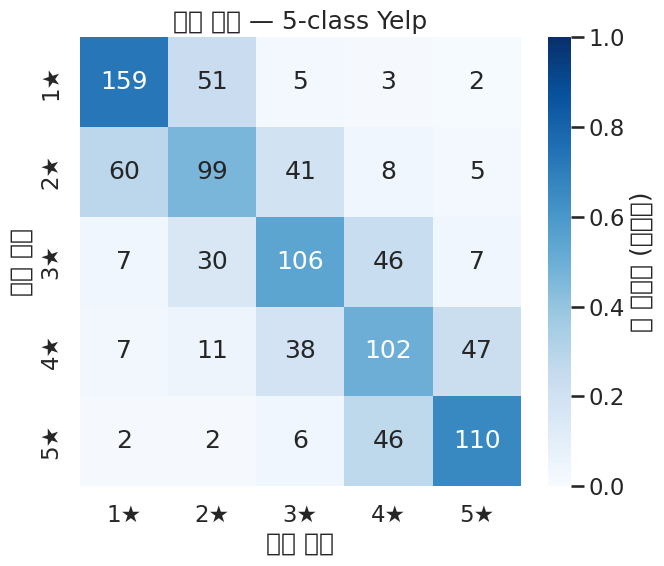
\includegraphics[width=0.76\linewidth]{assets/figures/ch12_confusion_matrix.png}
\end{bookfigurelabel}



\textbf{해석 가이드}

\begin{itemize}
\tightlist
\item
  색의 진하기는 \emph{행 정규화} (정답 클래스 안에서의 비율) --- 대각선 셀의 색이 그 클래스의 \emph{재현율} 입니다.
\item
  숫자는 \emph{원본 카운트} 라 클래스별 표본 크기도 같이 보입니다 --- 어떤 클래스에 모델 평가 표본이 적으면 통계적 노이즈가 큼을 인지.
\item
  \inlinecode{1★\ →\ 2★} 또는 \inlinecode{4★\ →\ 5★} 같은 \emph{±1 이웃 오류} 가 가장 흔할 것 --- 별점 회귀에 가까운 task의 자연스러운 양상. 별점 \emph{3★} 이 가장 어려울 가능성이 큰데, 이는 사람도 1★/2★보다 혼동하는 \emph{중간} 평가이기 때문.
\end{itemize}



\subsection{최상위 확률 분포}

K=5에서는 \emph{어느 한 클래스에 압도적인 자신감} 이 있는 경우와 \emph{2-3 클래스 사이에서 갈피를 못 잡는} 경우가 나뉩니다. 정답·오답을 구분해 그리면 모델 자신감이 \emph{얼마나 calibration 됐는지} 가 드러납니다.



\Needspace{26\baselineskip}
\begin{lstlisting}
df_top = pd.DataFrame({
    "top1_prob": top1_prob,
    "outcome":   np.where(correct, "correct", "wrong"),
})

fig, ax = plt.subplots(figsize=(9, 5))
sns.kdeplot(
    data=df_top, x="top1_prob", hue="outcome",
    fill=True, common_norm=False, alpha=0.5,
    palette={"correct": "#5BD17F", "wrong": "#E55050"},
    clip=(1/5, 1.0), ax=ax,
)
ax.axvline(1/5, color="black", lw=1.0, ls=":", alpha=0.5)
ax.text(
    1/5,
    ax.get_ylim()[1]*0.95,
    "  uniform = 1/K",
    va="top",
    fontsize=10,
    alpha=0.6,
)
ax.set_title("Top-1 probability — distribution split by correctness")
ax.set_xlabel("top-1 predicted probability  max_k P(y=k)")
ax.set_ylabel("Density")
plt.tight_layout()
plt.show()
\end{lstlisting}

\begin{bookfigurelabel}[htbp]{정답 여부에 따른 최상위 예측 확률 분포}{fig:ch12-top1-probability}
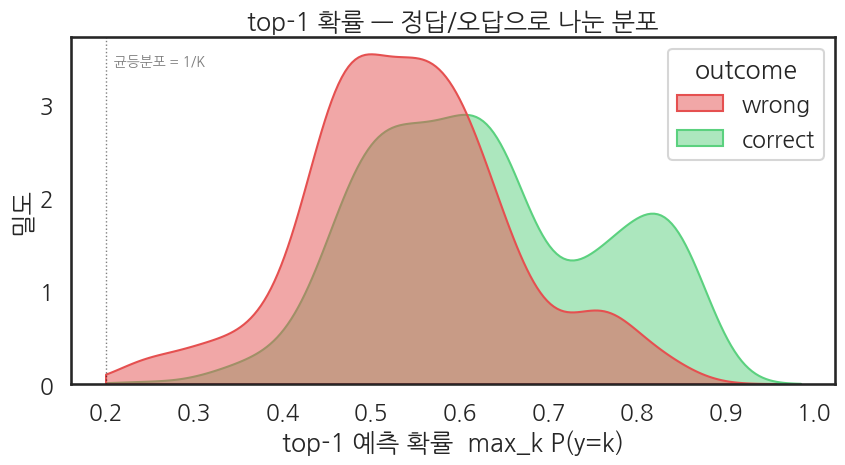
\includegraphics[width=0.88\linewidth]{assets/figures/ch12_top1_probability.png}
\end{bookfigurelabel}



\textbf{해석}

\begin{itemize}
\tightlist
\item
  \textbf{잘 학습된 모델}은 \emph{correct 곡선이 1.0 가까이} 몰리고 \emph{wrong 곡선은 더 낮은 영역} (0.4-0.7)에 퍼져 있습니다. 모델이 틀릴 때는 \emph{덜 자신 있게} 틀려야 calibration이 좋다는 뜻.
\item
  \textbf{두 곡선이 1.0 근처에서 함께 압착} 되어 있으면 → 모델이 \emph{틀린 답에도 매우 자신} 있는 \emph{over-confident} 상태. 별점 ±1 이웃 오류가 많을수록 이 현상이 도드라짐.
\item
  \textbf{correct 곡선이 0.5-0.8 근처에 머무르면} → 모델이 \emph{정답을 알면서도 망설이는} 상태. 학습이 부족하거나 task가 본질적으로 모호한 경우.
\end{itemize}



\Needspace{9\baselineskip}
\begin{lstlisting}
print(classification_report(
    labels, preds,
    target_names=[STAR_LABELS[k] for k in range(5)],
    digits=4, zero_division=0,
))
\end{lstlisting}



\section{BERT와 TF-IDF 비교}

같은 데이터에 \ref{ch:05}장 셋업(TF-IDF + multinomial LogReg)을 \emph{이 노트북 안에서} 다시 학습해 비교합니다. \textbf{BERT 67M 파라미터가 진짜로 도움이 되는가?} 가 이 비교의 핵심 질문 --- sklearn은 GPU 없이도 몇 초 만에 끝나기 때문에 self-contained로 부담 없이 포함됩니다.



\Needspace{26\baselineskip}
\begin{lstlisting}
texts_train  = list(train_full["text"])
labels_train = list(train_full["label"])
texts_eval   = list(eval_full["text"])
labels_eval  = list(eval_full["label"])

vec = TfidfVectorizer(
    max_features=20000,
    ngram_range=(1, 2),
)
X_train = vec.fit_transform(texts_train)
X_eval  = vec.transform(texts_eval)

clf = LogisticRegression(max_iter=2000, n_jobs=-1)
clf.fit(X_train, labels_train)

probs_sk = clf.predict_proba(X_eval)
# (B, 5)
preds_sk = probs_sk.argmax(axis=1)
# (B,)

acc_sk = float(accuracy_score(labels_eval, preds_sk))
ps, rs, f1s, _ = precision_recall_fscore_support(
    labels_eval,
    preds_sk,
    average="macro",
    zero_division=0,
)
auc_sk = float(roc_auc_score(labels_eval, probs_sk, multi_class="ovr"))

print(f"sklearn TF-IDF + LogReg:")
print(f"  vocabulary size:    {len(vec.vocabulary_):,}")
print(
    f"  trained parameters: {clf.coef_.size + clf.intercept_.size:,}  (~"
    f"{clf.coef_.size/1e3:.0f} K)"
)
print(f"  accuracy:           {acc_sk:.4f}")
print(f"  macro F1:           {f1s:.4f}")
print(f"  AUC (OvR):          {auc_sk:.4f}")
\end{lstlisting}



\subsection{평가지표 비교}



\Needspace{26\baselineskip}
\begin{lstlisting}
metrics_bert = {
    k.replace(
        "eval_",
        ""): v for k,
        v in eval_metrics.items(,
    )
    if k.startswith("eval_") and isinstance(v, float)
}
metrics_sk = {
    "accuracy":        acc_sk,
    "macro_precision": float(ps),
    "macro_recall":    float(rs),
    "macro_f1":        float(f1s),
    "auc_ovr":         auc_sk,
}

common = [k for k in metrics_bert if k in metrics_sk]
cmp = pd.DataFrame({
    "metric":             common,
    "sklearn (TF-IDF)":   [metrics_sk[k]   for k in common],
    "BERT":               [metrics_bert[k] for k in common],
})
cmp["BERT - sklearn"] = cmp["BERT"] - cmp["sklearn (TF-IDF)"]
print(cmp.round(4).to_string(index=False))
\end{lstlisting}



\subsection{혼동 행렬 비교}

같은 평가 데이터에 sklearn은 어디서, BERT는 어디서 혼동하는지 \emph{나란히} 봅니다.



\Needspace{26\baselineskip}
\begin{lstlisting}
cm_bert = confusion_matrix(
    labels,
    preds,
    labels=list(range(5)),
)
cm_sk   = confusion_matrix(
    labels_eval,
    preds_sk,
    labels=list(range(5)),
)

cm_bert_n = cm_bert / cm_bert.sum(axis=1, keepdims=True)
cm_sk_n   = cm_sk   / cm_sk.sum(axis=1, keepdims=True)

fig, axes = plt.subplots(1, 2, figsize=(13, 5.5))
for ax, cm_n, cm_raw, title in [
    (axes[0], cm_sk_n,   cm_sk,   "sklearn TF-IDF + LogReg"),
    (axes[1], cm_bert_n, cm_bert, "BERT"),
]:
    sns.heatmap(
        cm_n, annot=cm_raw, fmt="d", cmap="Blues", vmin=0, vmax=1,
        xticklabels=[STAR_LABELS[k] for k in range(5)],
        yticklabels=[STAR_LABELS[k] for k in range(5)],
        cbar=False, ax=ax,
    )
    ax.set_title(title)
    ax.set_xlabel("Predicted star")
    ax.set_ylabel("Actual star")
plt.tight_layout()
plt.show()
\end{lstlisting}

\begin{bookfigurelabel}[htbp]{sklearn TF-IDF와 BERT의 혼동 행렬 비교}{fig:ch12-confusion-compare}
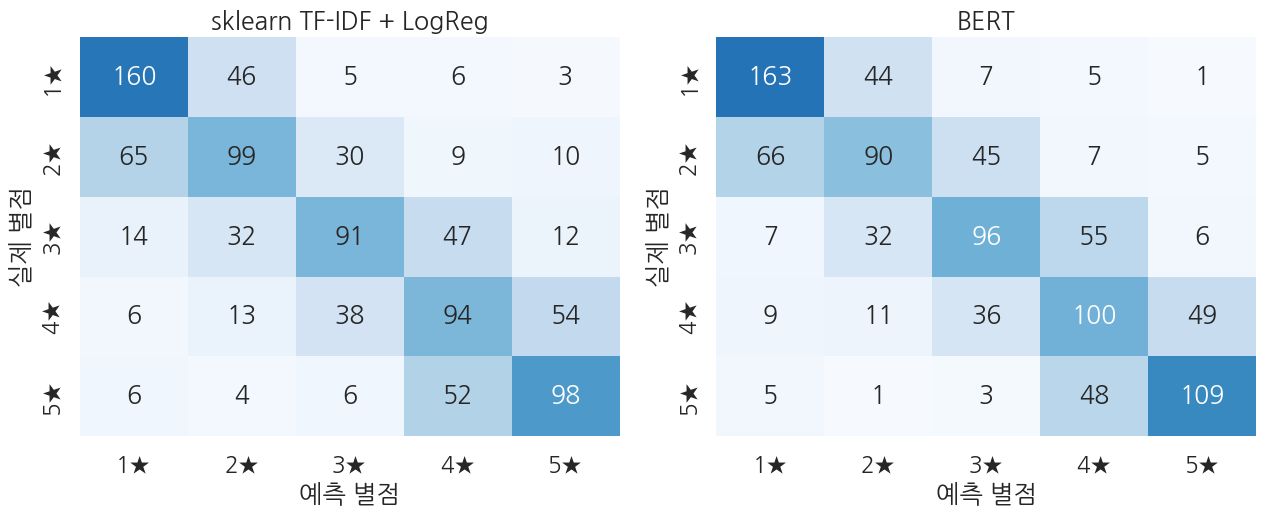
\includegraphics[width=0.96\linewidth]{assets/figures/ch12_confusion_compare.png}
\end{bookfigurelabel}



\textbf{해석 가이드}

\begin{itemize}
\tightlist
\item
  \emph{대각선이 더 진하면} 그 모델이 더 잘 맞춘 것.
\item
  \emph{인접 클래스 혼동(±1)} 은 두 모델 모두에서 가장 흔할 것 --- 별점이 \emph{순서형} 라벨이라 자연스럽습니다.
\item
  BERT가 sklearn 대비 가장 크게 개선되는 영역은 보통 \textbf{3★ (중간 별점)}: 단어 빈도만으로는 \emph{애매한 칭찬·비판이 섞인} 리뷰를 구분하기 어렵지만, BERT는 attention으로 문맥을 보기 때문.
\item
  만약 BERT가 sklearn보다 \emph{모든 셀에서} 비슷하거나 더 나쁘다면 → 학습량 부족 신호. epoch을 늘리거나 lr을 조정.
\end{itemize}



\section{이 장에 등장한 라이브러리·함수}

\begin{booktable}{12장 새로 등장한 라이브러리}{tab:ch12-06}
\begin{adjustbox}{max width=\textwidth}
\begin{tabular}{@{}lll@{}}
\toprule
이름 & 한 줄 설명 & 다음 장에서 \\
\midrule

\inlinecode{AutoModelForSequenceClassification(num\_labels=5,\ problem\_type="single\_label\_classification")} & \ref{ch:11}장 셋업에서 K만 5로 & \ref{ch:13}장에서 \inlinecode{multi\_label\_classification} 으로 K=5 multi-label 매핑 \\
\inlinecode{sklearn.metrics.confusion\_matrix} & 혼동 행렬 raw 카운트 & 분류 장마다 사용 \\
\inlinecode{seaborn.heatmap(annot=...,\ fmt="d")} & 혼동 행렬 시각화 (색은 비율, 숫자는 카운트) & 분류 장마다 동일 패턴 \\
\inlinecode{roc\_auc\_score(...,\ multi\_class="ovr")} & multi-class AUC를 One-vs-Rest로 계산 & 13·15장-18에서 multi-label / multi-class 평가 \\
\inlinecode{precision\_recall\_fscore\_support(...,\ average="macro")} & 클래스 불균형에서 모든 클래스에 같은 가중치 & 분류 장마다 등장 \\
\bottomrule
\end{tabular}
\end{adjustbox}
\end{booktable}



\section{체크포인트 질문}

\begin{enumerate}
\def\labelenumi{\arabic{enumi}.}
\tightlist
\item
  K=5에서 학습 시작 시 train loss가 약 1.6 정도라면 모델이 무엇을 학습한 상태인가요?
\item
  \emph{macro} F1과 \emph{micro} (= accuracy) 의 차이가 크다면 무엇을 의심해야 하나요?
\item
  혼동 행렬에서 ±1 이웃 클래스 혼동이 많다는 것은 무엇을 시사합니까?
\item
  BERT의 67M 파라미터가 sklearn의 \textasciitilde100K 파라미터(TF-IDF 5클래스)보다 정확도가 \emph{몇 \%p} 높다면 그 비용을 감수할 가치가 있다고 판단할 수 있나요?
\end{enumerate}



\section{FAQ}

\begin{faqBox}{Q1. (실무) BERT multi-class에서 클래스 불균형이 심하면 어떻게 하나요?}

가장 흔한 처치 두 가지:

\begin{enumerate}
\def\labelenumi{\arabic{enumi}.}
\tightlist
\item
  \textbf{\inlinecode{class\_weight} 적용} --- \inlinecode{Trainer.compute\_loss} 를 오버라이드해서 \inlinecode{CrossEntropyLoss(weight=...)} 를 명시적으로 사용. 가중치는 보통 \inlinecode{1\ /\ class\_count} 의 정규화 형태.
\end{enumerate}

\Needspace{15\baselineskip}
\begin{lstlisting}
from torch import nn

weights = torch.tensor([1.0, 1.5, 3.0, 1.2, 0.8]).to("cuda")
loss_fn = nn.CrossEntropyLoss(weight=weights)

class WeightedTrainer(Trainer):
    def compute_loss(self, model, inputs, return_outputs=False, **kwargs):
        labels = inputs.pop("labels")
        outputs = model(**inputs)
        loss = loss_fn(outputs.logits, labels)
        return (loss, outputs) if return_outputs else loss
\end{lstlisting}

\begin{enumerate}
\def\labelenumi{\arabic{enumi}.}
\setcounter{enumi}{1}
\tightlist
\item
  \textbf{데이터 단계 oversampling/undersampling} --- \inlinecode{imbalanced-learn} 의 \inlinecode{RandomOverSampler} 같은 도구로 학습 데이터를 균형있게. 단순하고 효과적.
\end{enumerate}

\end{faqBox}

\begin{faqBox}{Q2. (이론) softmax는 왜 \emph{상대 logit} 만 보나요? 그러면 절대 logit 값에 의미가 없나요?}

수식으로:

\begin{equation}
\label{eq:ch12-02}
\mathrm{softmax}(z + c \cdot \mathbf 1)_k = \dfrac{e^{z_k + c}}{\sum_j e^{z_j + c}} = \dfrac{e^{z_k} e^c}{e^c \sum_j e^{z_j}} = \mathrm{softmax}(z)_k
\end{equation}

식~\eqref{eq:ch12-02}은 이 절에서 사용하는 핵심 관계를 정리한 것입니다.

모든 logit에 같은 상수 \(c\) 를 더해도 softmax 출력이 동일합니다. 즉 K-차원 logit 벡터의 K-1 자유도만 학습됨 (K=5에선 4자유도).

\textbf{절대 logit 값은 \emph{학습 신호 크기} 를 결정}합니다. logit 값이 크면 (예: \(\vert{}z_k\vert{} \gg 1\)) softmax가 한쪽에 압착되어 gradient가 작아지고, 작으면 (예: \(\vert{}z_k\vert{} \approx 0\)) gradient가 균등해 모든 클래스가 학습됩니다. 학습 초기엔 logit이 작아 모든 클래스에 신호가 가는 게 좋고, 후반엔 logit이 커져 confident한 결정을 내리게 됩니다.

\end{faqBox}

\begin{faqBox}{Q3. (실무) eval 데이터에 어떤 클래스가 \emph{하나도} 안 나타나면 AUC 계산이 실패하는데 어떻게 하나요?}

\inlinecode{roc\_auc\_score(multi\_class="ovr")} 는 \emph{각 클래스에 대해} positive/negative를 나누어 AUC를 계산하는데, positive 샘플이 0개인 클래스가 있으면 AUC를 정의할 수 없어서 \inlinecode{ValueError} 가 납니다.

처치는 두 가지:

\begin{enumerate}
\def\labelenumi{\arabic{enumi}.}
\tightlist
\item
  \textbf{try/except로 NaN 반환} --- 이 장의 \inlinecode{compute\_metrics} 가 사용하는 패턴. 학습 자체엔 영향 없음.
\item
  \textbf{eval 데이터를 더 모아서 모든 클래스가 등장하도록} --- 운영 환경에선 이게 정석. 평가의 통계적 신뢰도 자체에도 도움.
\end{enumerate}

평가 셋이 1,000건 정도면 5클래스가 모두 등장할 가능성이 높지만, 각 클래스 표본이 \textasciitilde200건 안팎이라 통계 잡음이 큽니다. 가능하면 평가 셋을 늘리세요.

\end{faqBox}

\begin{faqBox}{Q4. (이론) 별점 1-5는 \emph{순서형 라벨} 인데 왜 회귀(\ref{ch:09}장) 대신 분류(\ref{ch:12}장)로 푸나요?}

둘 다 가능하고 각각 장단점이 있습니다.

\begin{booktable}{12장 FAQ 표}{tab:ch12-07}
\begin{adjustbox}{max width=\textwidth}
\begin{tabular}{@{}lll@{}}
\toprule
& 회귀 (\ref{ch:09}장 방식) & 분류 (\ref{ch:12}장 방식) \\
\midrule

라벨 의미 & 별점이 \emph{연속} 값 (1.0-5.0) & 별점이 \emph{5개의 명목 클래스} \\
손실 & MSE --- 4★ vs 5★ 차이 = (1)² = 1 & CE --- 4★ vs 5★ 차이도 1★ vs 5★ 차이도 \emph{같은 손실} \\
출력 & scalar 1.0-5.0 & (5,) 확률 벡터 \\
±1 인접 오류 페널티 & 작음 & 크지 않음 (정답 확률이 어느 정도 있으면) \\
모델이 \emph{순서} 를 인지? & \textbf{자동으로 인지} & 명시적으론 인지 안 함 (학습 데이터 통계로 우회 학습) \\
\bottomrule
\end{tabular}
\end{adjustbox}
\end{booktable}

\textbf{언제 어느 방식을?} 별점이 \emph{진짜 순서형이고 distance가 의미있다} (1★→5★는 1★→2★보다 4배 더 부정적) 면 회귀가 자연스럽습니다. 별점이 \emph{카테고리에 가까워서 distance 의미가 약하다} (예: 영화 장르 분류) 면 분류가 자연스럽습니다.

\textbf{ordinal regression} 이라는 별도의 분야가 있어 \emph{순서형} 의 특수 구조를 살리는 손실(예: cumulative link)을 씁니다. 입문 수준에선 다루지 않습니다.

\end{faqBox}

\begin{faqBox}{Q5. (실무) BERT가 sklearn 대비 \emph{조금만} 좋다면 BERT를 안 쓰는 게 나을까요?}

5-10\%p 정도 정확도 향상이라면 trade-off:

\begin{itemize}
\tightlist
\item
  \textbf{inference 비용}: BERT는 GPU 권장 (CPU에선 \textasciitilde50배 느림). sklearn은 CPU로 충분. 운영 비용 차이 5-10배.
\item
  \textbf{메모리}: BERT 모델 \textasciitilde250MB 디스크, \textasciitilde500MB 메모리. sklearn은 \textasciitilde10MB.
\item
  \textbf{학습 시간}: BERT는 GPU 5-10분. sklearn은 CPU 5-30초. 실험 cycle 100배 차이.
\item
  \textbf{유연성}: BERT는 fine-tune이 가능 (도메인 특화 추가 학습). sklearn은 \emph{처음부터 다시} 학습.
\end{itemize}

단순 \emph{정확도-vs-비용} 만 보면 \textbf{5\%p 이내 차이면 sklearn}, \textbf{10\%p 이상이면 BERT 고려} 같은 룰이 무난합니다. 별점 task처럼 \emph{단어 빈도가 강한 신호} 인 도메인은 sklearn 유리, \emph{부정·반어·다단계 추론} 이 중요한 NLI/감성분석 도메인은 BERT 유리.

\textbf{그런데 정확도 너머의 가치가 있습니다.} 다음 시나리오에서는 정확도 차이가 \emph{2-3\%p} 만 나도 BERT가 압도적으로 유리합니다 --- sklearn으로는 \emph{애초에 불가능} 하거나 별도 파이프라인을 통째로 다시 만들어야 하기 때문.

\textbf{(1) 새 도메인으로의 빠른 적응 --- \emph{transfer learning}}

영어 일반 리뷰로 학습한 BERT를 \emph{의료 환자 리뷰} 100-500건만으로 fine-tune해 즉시 도메인 모델을 얻을 수 있습니다. sklearn은 도메인이 바뀌면 \emph{어휘 통계가 처음부터 다시} --- 의료 용어 빈도가 일반 리뷰와 달라 TF-IDF가 새 분포에서 학습돼야 하고, 100건은 통계적으로 너무 적습니다.

\Needspace{6\baselineskip}
\begin{lstlisting}
model = AutoModelForSequenceClassification.from_pretrained("yelp-finetuned-bert")
model.train_on(medical_reviews_500)
\end{lstlisting}

\textbf{(2) 다국어 / cross-lingual --- 같은 코드로 한국어·일본어·영어}

\inlinecode{xlm-roberta-base} 같은 다국어 BERT는 \emph{동일 모델 + 동일 코드} 로 100+ 언어 동작. 영어 Yelp로 학습한 모델이 \emph{한국어 리뷰에도 그대로 generalize} 합니다 (zero-shot cross-lingual transfer). sklearn은 언어마다 토크나이저(형태소 분석기), 불용어 사전, TF-IDF vocabulary를 \emph{각각} 만들어야 합니다.

\Needspace{6\baselineskip}
\begin{lstlisting}
tok = AutoTokenizer.from_pretrained("xlm-roberta-base")
model.predict(tok("이 식당 음식이 정말 별로였어요"))
\end{lstlisting}

\textbf{(3) 분류 너머의 task로 확장 --- 같은 백본, 다른 헤드}

같은 \inlinecode{distilbert-base-uncased} 본체로:

\begin{booktable}{12장 FAQ 표}{tab:ch12-08}
\begin{adjustbox}{max width=\textwidth}
\begin{tabular}{@{}lll@{}}
\toprule
Task & 모델 클래스 & 예시 \\
\midrule

분류 (이 장) & \inlinecode{AutoModelForSequenceClassification} & 별점 1-5 분류 \\
토큰 분류 (NER) & \inlinecode{AutoModelForTokenClassification} & “\emph{Bob} 가 \emph{Apple} 에서 \emph{iPhone} 을 샀다” → 사람/회사/제품 추출 \\
질의응답 & \inlinecode{AutoModelForQuestionAnswering} & “이 리뷰의 만족도는?” 답: “음식은 좋지만 서비스가” \\
텍스트 생성 & \inlinecode{AutoModelForCausalLM} & 자동 답변 생성 \\
임베딩 & \inlinecode{AutoModel} (CLS hidden state) & 문장 의미 벡터 \\
\bottomrule
\end{tabular}
\end{adjustbox}
\end{booktable}

sklearn LogReg는 \emph{분류 한 가지} 만. 다른 task는 모델 자체가 달라져야 합니다.

\textbf{(4) 임베딩 기반 의미 검색·중복 제거}

BERT {[}CLS{]} 임베딩은 \emph{문장 의미를 768-dim 벡터} 로 만듭니다. 단어가 달라도 \emph{의미가 비슷하면 가까운 벡터}. TF-IDF는 \emph{같은 단어} 가 있어야 매칭 --- “맛있다” 와 “delicious” 는 거리 1, BERT는 거의 거리 0.

\Needspace{8\baselineskip}
\begin{lstlisting}
emb1 = model(tok("맛있고 친절했어요"))[:, 0, :]
# CLS
emb2 = model(tok("음식 훌륭하고 직원 좋았음"))[:, 0, :]
cos_sim(emb1, emb2)
\end{lstlisting}

리뷰 수만 건 중 \emph{의미 중복} 을 제거하거나, 새 리뷰가 들어왔을 때 \emph{비슷한 과거 리뷰} 를 검색하는 시스템 --- sklearn으로는 거의 불가능.

\textbf{(5) Zero-shot 분류 --- 학습 데이터 없이도 동작}

NLI(natural language inference)로 fine-tune된 BERT (\inlinecode{facebook/bart-large-mnli} 등)는 \emph{임의의 라벨} 에 대해 학습 \emph{없이} 분류합니다.

\Needspace{15\baselineskip}
\begin{lstlisting}
from transformers import pipeline
zsc = pipeline(
    "zero-shot-classification",
    model="facebook/bart-large-mnli",
)
zsc(
    "음식이 별로였다",
    candidate_labels=["positive", "negative", "neutral"],
)
# {"labels": ["negative", "neutral", "positive"], 
# "scores": [0.91, 0.07, 0.02]}
\end{lstlisting}

새 라벨 카테고리가 생길 때마다 학습 데이터 라벨링 비용이 없습니다. 빠른 프로토타이핑·콜드스타트에 강력. sklearn은 \emph{학습 데이터 필수}.

\textbf{정리} --- sklearn은 \emph{오늘의 task} 를 가장 빠르고 싸게 푸는 도구. BERT는 \emph{task 자체가 진화하거나, 도메인이 늘어나거나, 분류 외 응용으로 확장될 때} 의 자산. 정확도 비교만으로 BERT 가치를 판단하기 부족한 이유입니다.

\end{faqBox}

\begin{faqBox}{Q6. (실무) 한 모델로 \emph{binary와 5-class를 동시에} 풀 수 있나요?}

\textbf{multi-task learning} 이라는 패턴으로 가능합니다.

\Needspace{22\baselineskip}
\begin{lstlisting}
class MultiTaskModel(nn.Module):
    def __init__(self, backbone):
        super().__init__()
        self.backbone = backbone
        self.head_binary = nn.Linear(768, 2)
        # binary head
        self.head_5class = nn.Linear(768, 5)
        # 5-class head

    def forward(self, **inputs):
        h = self.backbone(**inputs).last_hidden_state[:, 0]
        # CLS
        return {"binary": self.head_binary(h), "5class": self.head_5class(h)}

loss = ce(
    out["binary"],
    y_binary) + ce(out["5class"], y_5class,
)
\end{lstlisting}

DistilBERT body가 \emph{공유} 되어 두 task가 서로의 학습에 도움을 줍니다. \ref{ch:14}장 (Auxiliary Loss)에서 비슷한 패턴을 본격적으로 다룹니다.
\end{faqBox}



\section{오류 실험 (선택)}

다음 코드를 돌려보면 어떤 에러가 날까요?

\Needspace{17\baselineskip}
\begin{lstlisting}
def tokenize_wrong(batch):
    out = tokenizer(
        batch["text"],
        truncation=True,
        max_length=128,
    )
    onehot = []
    for l in batch["label"]:
        v = [0.0] * 5
        v[l] = 1.0
        onehot.append(v)
    out["labels"] = onehot
    return out
\end{lstlisting}

힌트: \inlinecode{single\_label\_classification} + \inlinecode{CrossEntropyLoss} 가 받는 라벨은 \emph{int 인덱스 1차원 텐서} (shape \inlinecode{(B,)})인데 위 코드는 \emph{(B, 5)} 형태를 넘깁니다. multi-label 형식의 라벨을 single-label 모델에 넣으려는 흔한 실수.



\begin{previewBox}{미리보기: 다음 장}

\textbf{\ref{ch:13}장. BERT 다중 라벨 분류 (Multi-label \& Per-label BCE)}

\begin{itemize}
\tightlist
\item
  같은 BERT, 같은 데이터에 \emph{측면(food/service/price/ambiance/location) 키워드 자동 라벨링} 추가
\item
  \inlinecode{num\_labels=5} 그대로 (\ref{ch:12}장과 같음), 단 \inlinecode{problem\_type="multi\_label\_classification"} 으로 전환
\item
  Activation은 (per-label) sigmoid, Loss는 (per-label) \inlinecode{BCEWithLogitsLoss}
\item
  한 리뷰에 \emph{여러 측면이 동시에 등장} 할 수 있음 --- single-label과 본질적으로 다른 task
\item
  \ref{ch:06}장의 sklearn \inlinecode{OneVsRestClassifier(LogisticRegression)} 의 BERT 버전
\end{itemize}

\begin{quote}
\textbf{변하는 축}: \ref{ch:12}장 → \ref{ch:13}장 은 \emph{Loss 축} (CE → BCE per-label)이 변합니다 --- task가 \emph{single-label} 에서 \emph{multi-label} 로 바뀌는 것이 본질이고 그에 맞춰 loss/activation/라벨 형식이 동시에 따라옵니다.
\end{quote}
\end{previewBox}
